\section{Discussion}
A Wizard of Oz study has been conducted following the A-B-C-B design.  In Phase A, the parent alone prompted the child through hand-washing steps.  In first Phase B, the robot alone prompted the child.  In Phase C, the parent and the robot jointly prompted.  Visual analyses were used to analyze the measures from annotated video data of the trials.

%To evaluate the effectiveness of the robot prompts on child's step completion, to measure the child's compliance to the prompts, and to investigate their relationships with the child's engagement level during hand-washing, the following metrics are calculated and analyzed from the video data annotations for each trial:

%- was the robot more effective in guiding child to complete steps than the parent?
%- does the child respond to the robot equally well as to the parent?
%- is it because child is not engaged?  or is it because robot prompts not understandable? or is it because robot not as authoritative as the parent? or is it something else? (like not responsive enough, or not contingent to child's behaviour enough?)

\subsection{Primary Results}
We saw that having the robot present in the washroom contributed positively in increasing the Number of Complete Steps.  Comparing with the parent's prompts' contribution, the robot prompts had the similar size of contribution in the first Phase B, smaller size in Phase C, and bigger size in the second Phase B.  It is interesting that the robot had drastically greater contribution in the second Phase B (increase of 1.5), but not in the first (increase of 0.5).  We believe this is mainly due to the child learning to follow the robot after going through Phase C, where the parent jointly prompted with the robot, telling the child to follow the robot's prompts.  Although robot prompts in the second Phase B (increase of 1.5) did not arrive at the same effectiveness as that of the parent's in Phase A (increase of 3), we believe that, given sufficient Phase C training, the robot potentially could replace the parent as an independent prompting agent.

Another way to look at the robot prompts' effectiveness is this: We first observe that the Number of Incomplete Steps are kept near zero in all trials through either parent prompts or robot prompts or joint (Number of Incomplete Steps is shown in Figure \ref{fig:4NumberofIncompleteSteps}).  In addition, we saw that the Number of Parent Prompts - Overall was sharply reduced in both of B phases (when robot prompted alone) and experienced a continual reduction in Phase C when robot and parent jointly prompted.  This shows two things: First, in the two B phases, the robot was able to guide the child through hand-washing without constant parent supervision.  Second, in Phase C, when the parent jointly prompts with the robot to have the child better follow the robot, the parent was able to gradually fade out the prompts while keeping Number of Incomplete Steps near zero since the child listened to the robot more and more.
\begin{figure} [h]
	\centering
	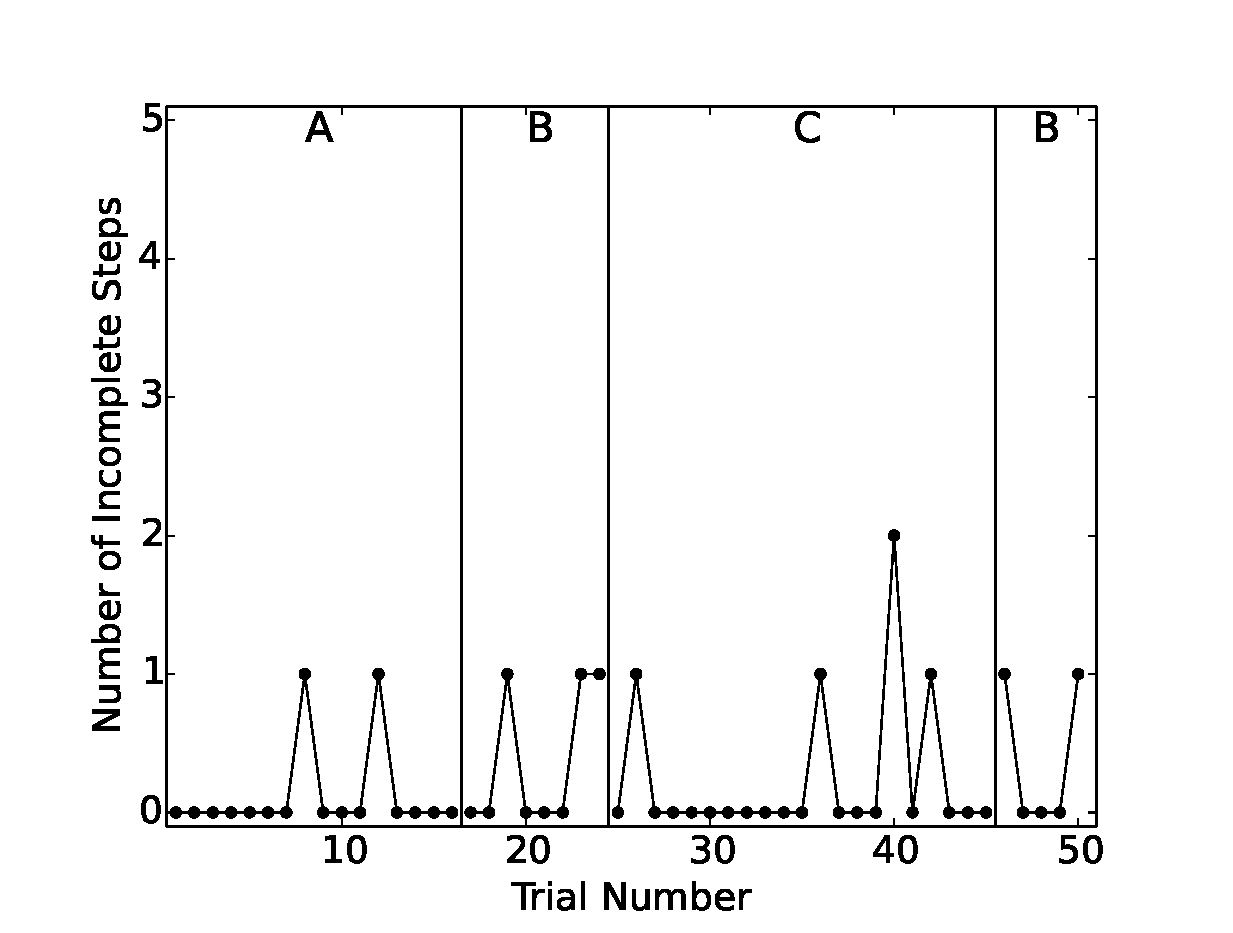
\includegraphics[width=0.6\textwidth]{./img/data_analysis/4NumberofIncompleteSteps.eps}
	\caption{Number of Incomplete Steps}
	\label{fig:4NumberofIncompleteSteps}
\end{figure}

One major limitation of evaluating robot prompt effectiveness based on the above measures (i.e. Number of Complete Steps and Number of Parent Prompts) is that we could have a trial where the child may be ignoring robot prompts and skipping steps.  This would fluctuate the total number of steps, and thus fluctuating Total Number of Complete Steps as well, influencing the estimation of effectiveness of robot vs. parent prompts.  Such fluctuation is not detectable using the measure Number of Parent Prompts, either.  Our study did not employ a strict hand-washing steps ordering that the child must adhere to, and we left it up to the parent's discretion to intervene as they think the child needs.  As a result, the measure Number of Parent Prompts does not fully reflect child skipping steps either.  One way to circumvent this problem may be to define a step order before hand, and monitor the measure Total Number of Steps Skipped each trial to characterize its effects.  However, it seems that children with ASD, or at least the one participant we had, had strict preference on the order of hand-washing steps, and the order is not known a priori and may be different across individuals.  Thus, having a flexible prompting scheme in terms of step orders is preferred.  However, this means that the decision of what steps need to be executed, and hence which steps were missed, often depends on the sequence of steps executed thus far in a trial.  This makes it troublesome to define what is meant by missed steps, possibly making the analysis process unfeasible.  Another way to circumvent this problem is to use other measures that reflect the child skipping steps, or not following the step order prompted -- the Compliance Rate and Not Affected By Prompt Rate measures can be used for this purpose.

We saw that both Compliance Rate and Hard Compliance Rate are high in Phase A, C, and second Phase B, and low in the first Phase B.  The contrary pattern exists for Not Affected By Prompt Rate.  This means that the prompts in the first Phase B were complied much less often, and a large portion of that noncompliance was exhibited as the child ignoring the prompts and kept doing some other step or not doing any step at all.  At the same time, both the Total Number of Complete Steps - With Robot and Parent Prompts and the Number of Parent Prompts - Overall are low in the first Phase B while the Number of Incomplete Steps in that phase is still near zero.  This is precisely the scenario talked about earlier, where the child skips many steps while the parent did not enforcement the steps skipped through prompts.  Thus, it is apparent that the robot was only effective in the second Phase B, but not in the first Phase B.  We believe the difference between first and second Phase B is that second Phase B is after Phase C, and first Phase B is before Phase C.  Phase C functioned as a training phase and helped the child comply better to robot prompts.

There are also other differences that existed between first and second Phase B, so training Phase C may not be the reason (or may not be the sole reason) for improved effectiveness of robot prompts in the second Phase B.  One important change happened to the way the robot was controlled starting at the seventh trial of first Phase B.  We found out, after introducing the robot to the child and conducting six trials, that the child did not follow the order of steps prompted by the robot.  This meant the robot needed to change the order of steps being prompted on the fly quickly.  However, due to the way its remote control was programmed, the researcher cannot change prompts quickly enough, resulting in the child growing impatient and ignored the robot prompts altogether.  Thus, the robot remote control scheme was changed from being inflexible in step order into one that the researcher can select the current prompting step on the fly.  Also, instead of implementing a timer, and automatically issuing the prompt after a predefined seconds of waiting, the timing of prompt delivery was changed to be decided by the researcher on the fly.  This makes the robot behavior much more flexible and relevant to the child's behaviors.  This robot control scheme change affected the last two trials in the first Phase B, and all trials in the second Phase B and Phase C.  This change, however, did not cause any abrupt change in any of our measures (comparing the last two trials of first Phase B with the previous trials in the phase).  Thus, we believe the robot control scheme change was not the cause of the improved effectiveness of robot prompts in the second Phase B.

It is important to mention here that the parent did not prompt the same way uniformly through Phase C, but instead was involved in various degrees.  The level of involvement was left up to the parent's discretion for each trial, with the ultimate goal to fade out the involvement to minimal by the end of Phase C.  By reviewing how the parent prompted the child, five levels of involvement were observed:
\begin{itemize}
	\item \textbf{Level 0}: the parent is outside of the room out of the child's view, only comes into the washroom to prompt when the child is not following the robot (this behavior is similar to that during Phase B)
	\item \textbf{Level 1}: the parent stands beside the child in the washroom, and mainly uses gestures to prompt the child to follow the robot and to demonstrate the step's motions after robot prompts
	\item \textbf{Level 2}: the parent stands beside the child in the washroom, and uses both verbals and gestures to prompt the child about each hand-washing steps, in competition to the robot prompts
	\item \textbf{Level 3}: the parent stands behind the child, and physically guide the child to follow the robot prompts
	\item \textbf{Level 4}: the parent stands beside the child, and prompts as the parent sees fit each hand-washing steps, with no robot present
\end{itemize}
The Parent Involvement Level is plotted in Figure \ref{fig:107ParentInvolvement}.  We see that, in Phase C, the parent mainly alternated between trial segments of level 1 and level 3 to train the child to follow the robot, while mixing single trials of level 0 to monitor the child's progress when left with robot alone.
\begin{figure} [h]
	\centering
	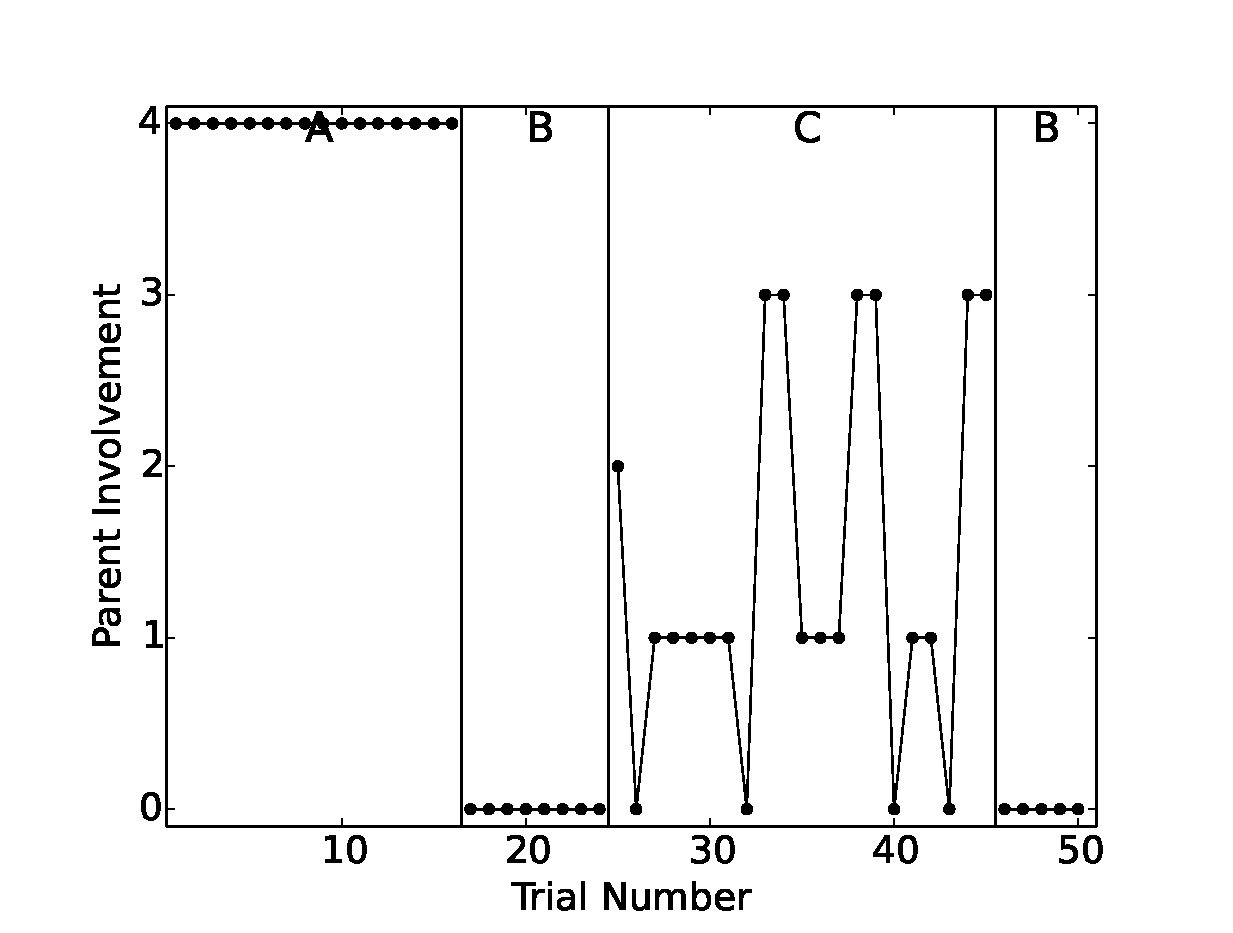
\includegraphics[width=0.6\textwidth]{./img/data_analysis/107ParentInvolvement.eps}
	\caption{Parent Involvement}
	\label{fig:107ParentInvolvement}
\end{figure}

With this in mind, we can attempt to answer what happened in Phase C that resulted in an increase of robot prompts effectiveness in the second Phase B.  The first observation we can make is by plotting only the level 0 parent involvement trials, where the robot is left alone with the child.  The Compliance Rate and Hard Compliance Rate for robot alone trials is shown in Figure \ref{fig:ComplianceRate_robotAloneOnly}.  The Not Affected By Prompt Rate for robot alone trials is shown in Figure \ref{fig:99NotAffectedByPromptRate-Overall_robotAloneOnly}.  We see a sharp jump rather than a gradual change in both Compliance Rate and Not Affected By Prompt Rate when we move from first Phase B to Phase C.  This suggests that the cause of effectiveness improvement of robot prompts was probably not a gradual processes such as the child learning hand-washing or getting used to the robot or washroom environment.  Instead, it was a sudden event experienced at the start of Phase C -- the joint prompting from the parent telling the child to follow the robot.  We also believe that, although the improvement in robot prompt effectiveness was immediate, a longer training Phase C was needed for the child to retain the behavior.  Note that Hard Compliance Rate did not show immediate change in levels.  This is possibly due to its low sample size, since hard compliance scenarios (child attempted a step before prompt and then was prompted for another step) were not that abundant.
\begin{figure}[h]
	\centering
	\begin{subfigure}[b]{0.49\textwidth}
		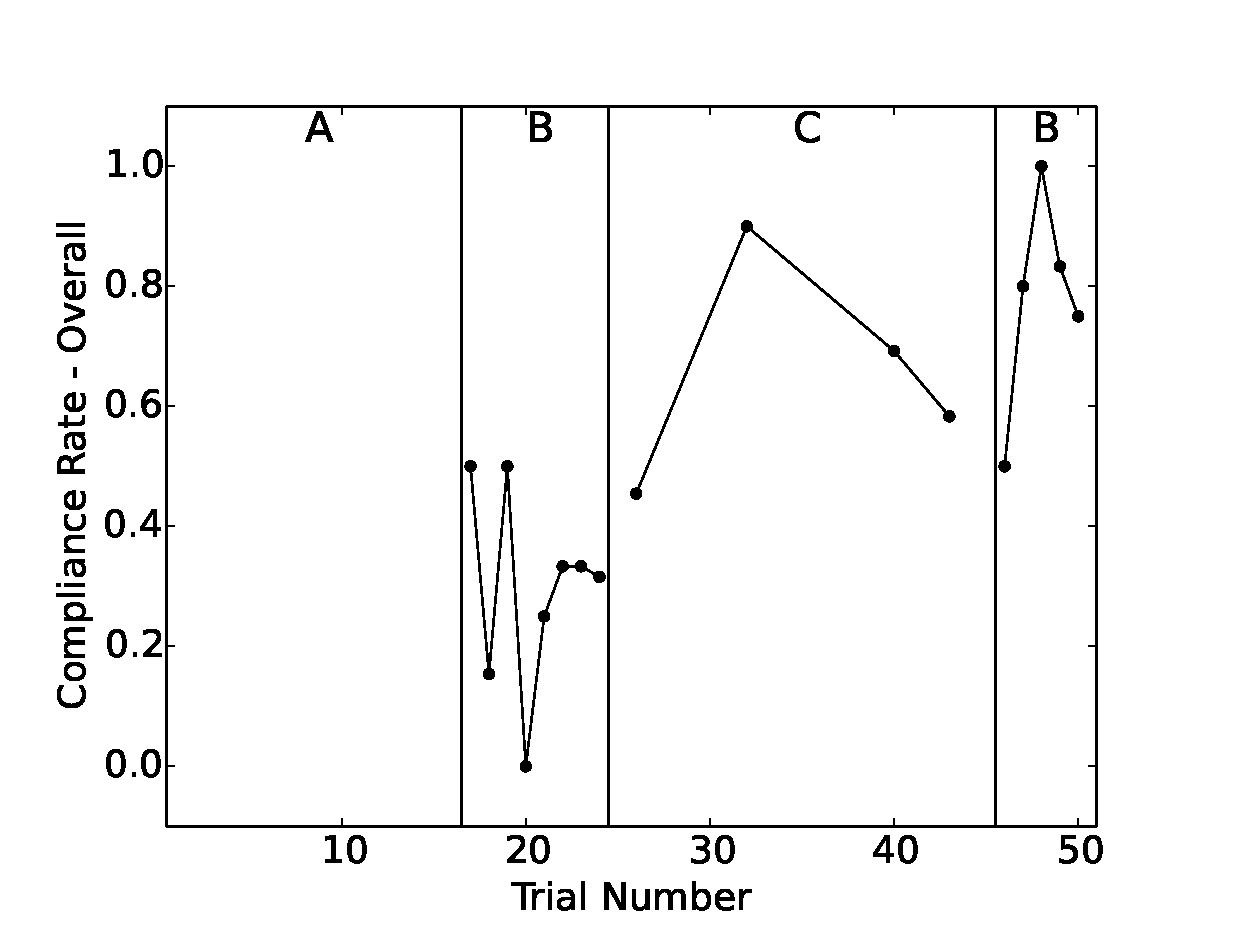
\includegraphics[width=1.1\linewidth]{./img/data_analysis/102ComplianceRate-Overall_robotAloneOnly.eps}
		\caption{Compliance Rate - Overall - Robot Alone Trials}
		\label{fig:102ComplianceRate-Overall_robotAloneOnly}
	\end{subfigure}
	\hfill
	\begin{subfigure}[b]{0.49\textwidth}
		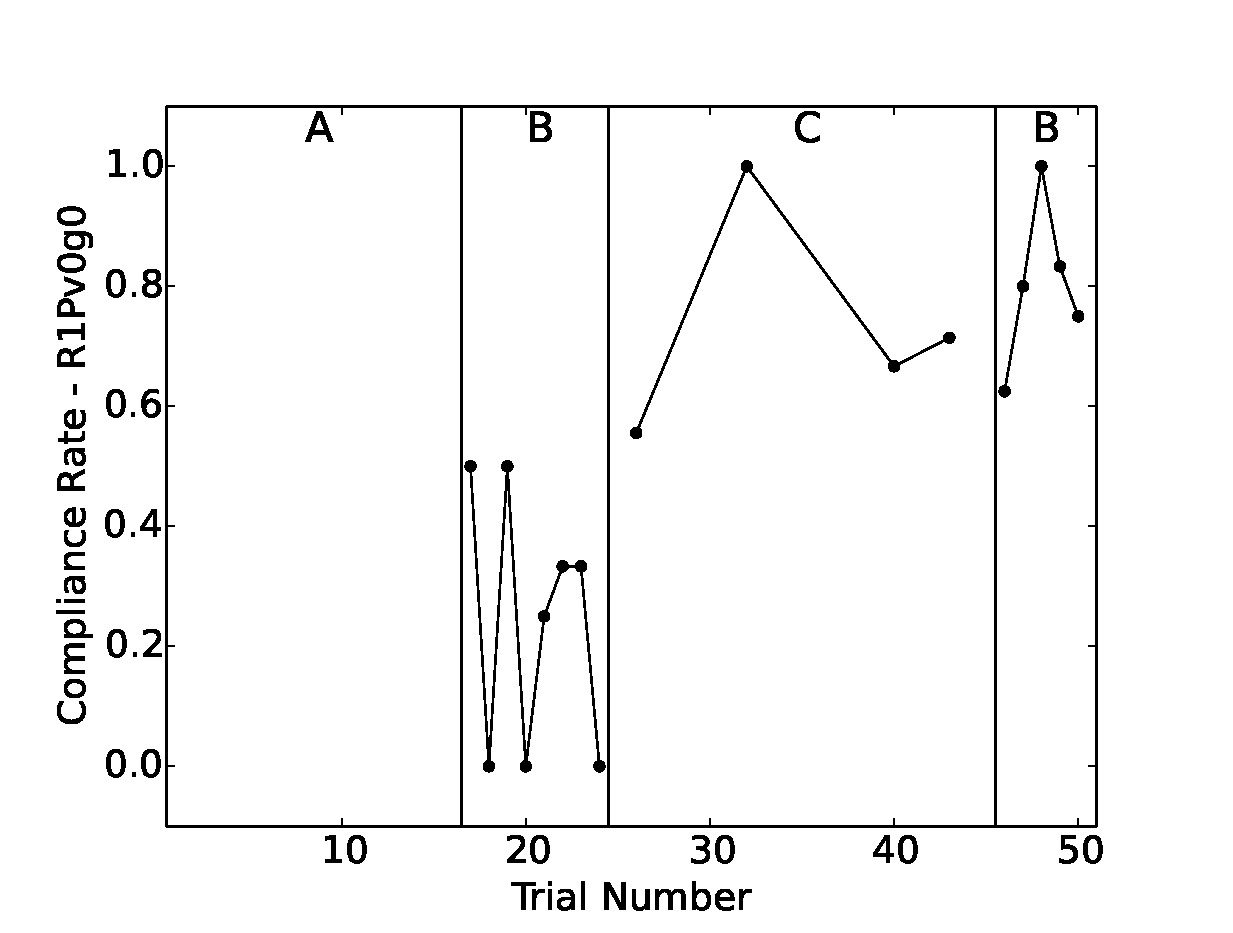
\includegraphics[width=1.1\linewidth]{./img/data_analysis/79ComplianceRate-R1Pv0g0_robotAloneOnly.eps}
		\caption{Compliance Rate - Robot Only Prompts - Robot Alone Trials}
		\label{fig:79ComplianceRate-R1Pv0g0_robotAloneOnly}
	\end{subfigure}%
	
	
	\begin{subfigure}[b]{0.49\textwidth}
		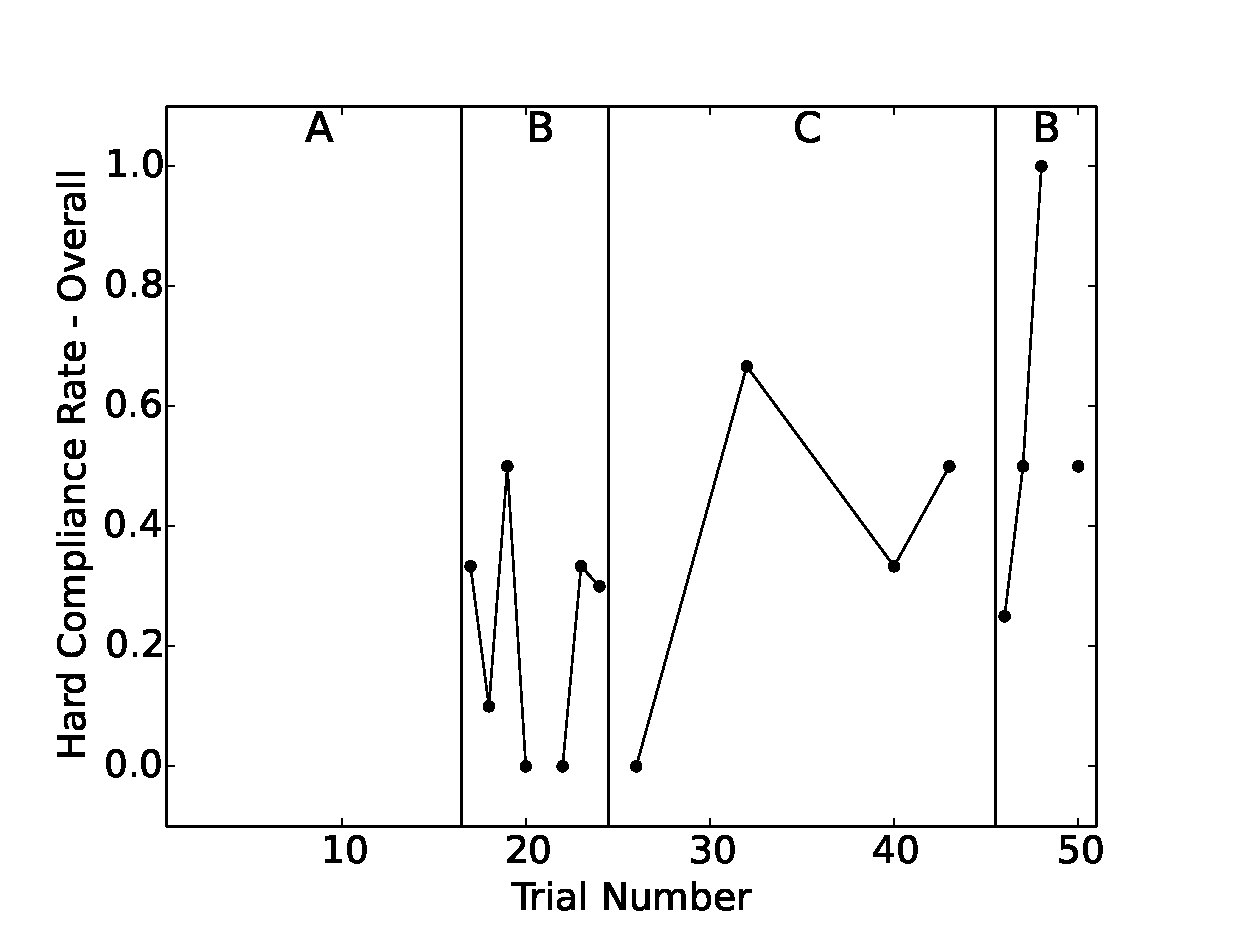
\includegraphics[width=1.1\linewidth]{./img/data_analysis/103HardComplianceRate-Overall_robotAloneOnly.eps}
		\caption{Hard Compliance Rate - Overall - Robot Alone Trials}
		\label{fig:103HardComplianceRate-Overall_robotAloneOnly}
	\end{subfigure}
	\hfill
	\begin{subfigure}[b]{0.49\textwidth}
		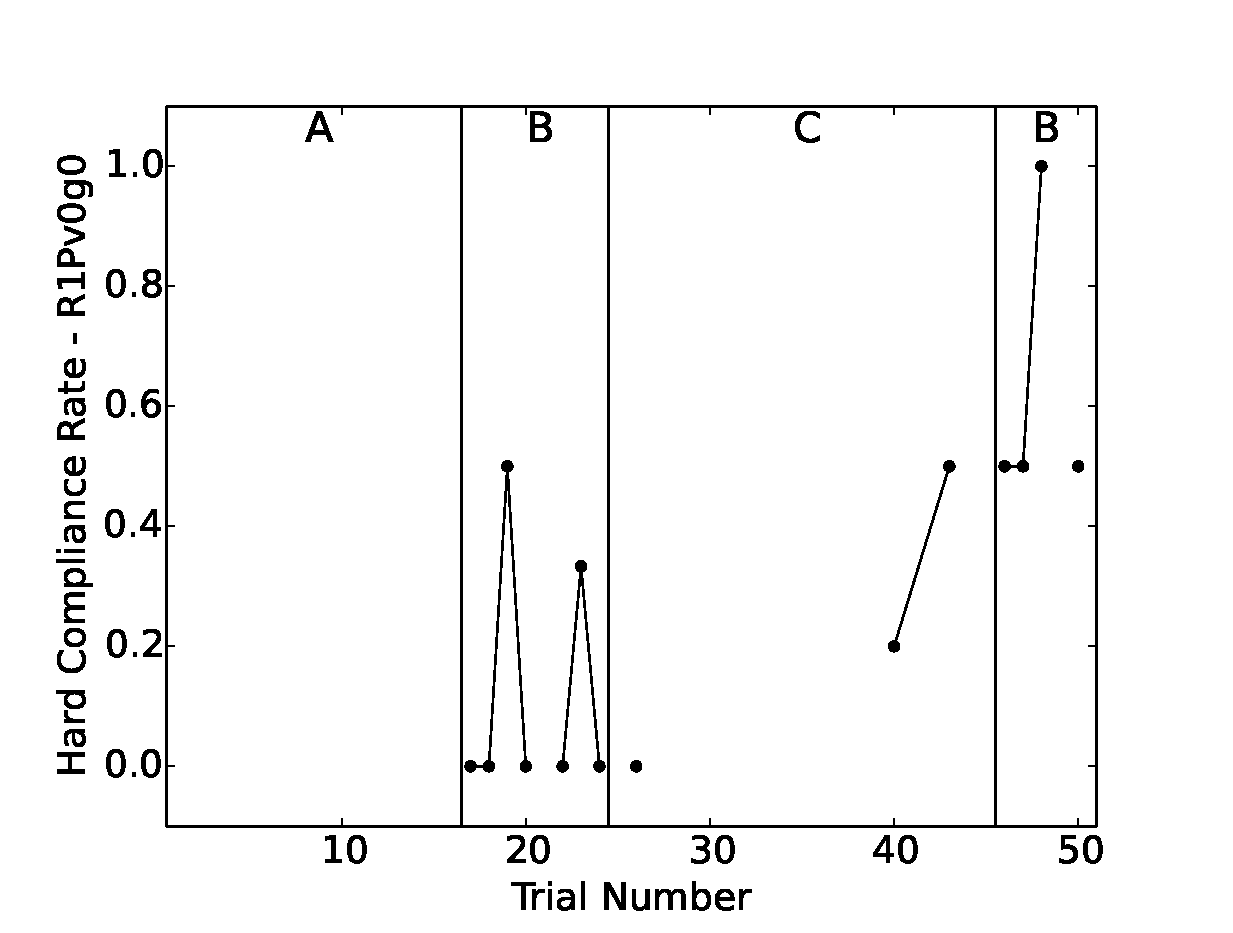
\includegraphics[width=1.1\linewidth]{./img/data_analysis/92HardComplianceRate-R1Pv0g0_robotAloneOnly.eps}
		\caption{Hard Compliance Rate - Robot Only Prompts - Robot Alone Trials}
		\label{fig:92HardComplianceRate-R1Pv0g0_robotAloneOnly}
	\end{subfigure}%
	\caption{Compliance Rate}
	\label{fig:ComplianceRate_robotAloneOnly}
\end{figure}
\begin{figure} [h]
	\centering
	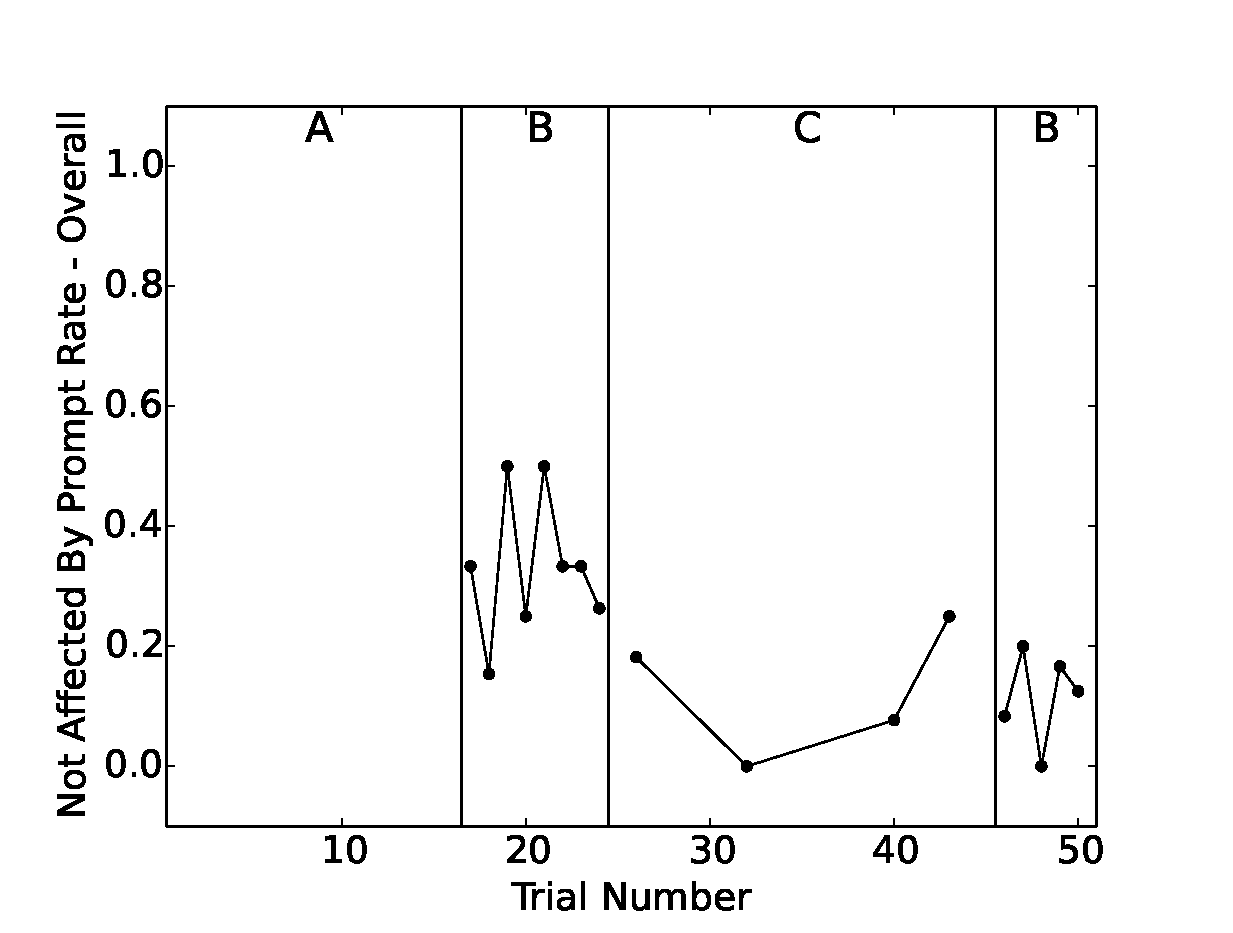
\includegraphics[width=0.6\textwidth]{./img/data_analysis/99NotAffectedByPromptRate-Overall_robotAloneOnly.eps}
	\caption{Not Affected By Prompt Rate - Robot Alone Trials}
	\label{fig:99NotAffectedByPromptRate-Overall_robotAloneOnly}
\end{figure}

As a summary of our primary results, we found that the robot was effective in guiding the child with ASD through hand-washing steps.  This was seen by a increased Number of Complete Steps and reduced Number of Parent Prompts as well as a maintained level of Prompt Compliance Rate.  Furthermore, we found that the child's compliance to robot prompts was not ideal when the robot was first introduced.  Through a training phase of the parent telling the child to follow the robot, the compliance rate was immediately improved.

\subsection{Secondary Results}
In addition to investigating the child's compliance in different intervention phases, we also attempted to characterize the child's engagement level, and possibly draw a causal link between higher engagement level and greater compliance.  We used measures Number of Times Child Smiles, Number of Times Child Murmurs, and Looking at Parent / Robot Rates (see Section \ref{sec:measures} for definitions) to characterize the child's engagement level during prompts and task executions.  However, we did not observe a correlation between any of these measures to the child's compliance rate.

The Number of Times Child Smiles did have a low level in First Phase B compared to Phase C and Second Phase B, but the level in Phase A should have been higher to be correlated with Compliance Rate.  Thus, although we can say the child tends to smile more in the later two phases, indicating that the child is more relaxed and having more fun, we can not draw a link between having fun and better compliance to prompts.

The Number of Times Child Murmurs did have a low level in First Phase B compared to Phase A and Phase C, but the level in Second Phase B should have been higher to be correlated with Compliance Rate.  What we found was that the child tends to murmur for two major reasons: in repeating the verbal prompt heard when the child is very engaged, and in protesting to the parent when the child does not wish to execute as prompted.  Thus, one could argue that this measure is not an ideal indicator for child's engagement level.  We also observed that the target to whom the child murmured to was often the parent, not the robot.  This may suggest that the child did not view the robot as a person one can communicate with, or that the child viewed the parent as the authoritative figure to appeal to in protest, not the robot.

The Looking at Robot Rate - Given Robot Prompted showed a high level in First Phase B, but decreased in the later two phases.  This is in contrary to the Compliance Rate, so no correlation was observed.  However, in comparison with Looking at Parent Rate and Given Both Prompted, we saw that the child prefers looking at the parent more than looking at the robot.  Also, the child looked at the robot more in the beginning of trials, but as trials went on, looked at the robot less.  This may be due to the robot not having a visually appealing appearance to the child.  The parent in Post-Intervention Survey also reported a lower level of satisfaction towards the robot's physical appearance.  Also, the appeal of the robot to the child may lie in not only its static appearance, but also the dynamics of its gestures and facial expressions.

\subsection{Limitations and Future Works}
Our Wizard of Oz study had many limitations.  The biggest one was having only one participant in the study.  This means our results maybe only applicable to this particular child, but not generalizable to the whole children with ASD population.  The next study in the future should increase the number of participants (maybe around ten subjects) while validating the major results of the current study.  The single subject research design should be used for this future study, since due to the diverseness of the children with ASD population, measures may have different levels across subjects.  Thus, we should generalize the effectiveness of an intervention by comparing the amount of change of measure levels for each child when having the intervention compared against him / her not having the intervention.  Also, the secondary aim of this future pilot study is to find out the participant demographics of a subpopulation of children with ASD that our intervention works consistently well on.  Only after this future study validating our major results and after we choose a subpopulation to focus on, should we attempt a larger scale (maybe around thirty subjects) randomized control trial, in which we divide the participants into control and intervention groups, and generalization of intervention effectiveness is made by directly comparing the measure levels between groups.  The focus of this randomized control would be to show clinical effectiveness of our intervention on the focused subpopulation.

Qualitative visual analysis was employed for the current study, where measure levels and trends were eyeballed.  We chose this analysis method due to its convenience, while accepting its inaccuracy as one of our limitations.  We felt that this inaccuracy is acceptable at the current stage of research -- having only one subject, with relatively few number of trials, and large noise in our measures.  However, as we move to the two future experiments mentioned above, quantitative analyses would be essential.  The pilot study could also employ visual analysis to make results comparable with the current study.  However, the randomized control trials study should strictly employ quantitative analysis only.

Another limitation was the reported change of robot control scheme in the middle of the First Phase B.  The reason for change was because our participant required a much more reactive robot who can switch the current step being prompted on the fly.  We felt the change was essential -- both the parent and the robot operator (the researcher) felt the robot was more responsive to the child after the control scheme switch.  However, the parent did report that the robot was still too slow for the child, and sometimes the pause between robot actions were too long.  We expected to see a change of measure levels due to robot scheme change.  However, due to noise in our measures, we could not observe such change.  Instead, only the change due to the parent robot training phase (Phase C) was apparent despite noise.  We felt the robot control scheme change was acceptable, since the focus of the current study is explore the possible questions and issues we might face In future experiments.  Thus, in future experiments we require the robot control scheme to be fixed.

Relating to the previous limitation was the fact that the current study (Wizard of Oz) involved a human operator (the researcher) remotely controlling the robot.  The researcher had no experience guiding the participant through hand-washing prior to the trials, and thus it was a learning process for the researcher through out the trials as well.  This meant that the researcher changed the order of steps the robot prompts were delivered to best fit the child's preference (e.g. the child preferred to put on soap before turning on water).  Also, the researcher chose prompts that were more effective (e.g. the attention grabber was not effective and so was not used in the end, and the child did not distinguish between scrub hands and rinse hands, so scrub hand prompts were not used in the end).  These changes were gradual, but may play a confounding effect on our measures.  However, we believe our major results, which reported an immediate change in Phase C, still stands despite the operator's learning effects.  One thing this does affect, though, is that in the future when we are automating the robot behaviors, tuning the robot prompts and order of steps to each child's preference is an inevitable task part of the automation process.

There are many sources of noise in the measures of the current study.  One of them is from the annotator(the researcher)'s subjectiveness when annotating the videos.  The annotator subjectivity may influence the different measures in varying degrees.  For example, when the parent repeats a verbal prompts several times in a roll, it is up to the annotator's discretion how many verbal prompts were issued.  Also, when the child executes a step almost simultaneously as a prompt is delivered, it is up to the annotator's discretion whether the prompt counts towards getting the child to execute the step.  Lastly, due to occasional obstruction of view and audio noise from running water, it is sometimes hard for annotator to tell whether the child smiles, murmurs, and looks at prompting parent / robot from the video.  All of the above are accepted as limitations of the current study, but can be improved through a more rigorous video annotation framework and better placement of video camera.  In addition, in future studies, the degree of annotator subjectiveness can be characterized by an inter-rater agreement measure such as the Cohen's Kappa \cite{volkmar2005handbook}.

Other confounding variables that produced measurement noise includes the following: First, the child was learning and getting better at hand-washing.  Although the child knew how to execute most of the hand-washing steps, he improved in remembering which step is next better through the trials, making him less and less dependent on prompts.  Second, the child's performance was influenced because he was new to the HomeLab washroom environment, which he gradually got used to the more he visited the lab.  The above two sources of noise can be reduced in future experiment through better control and maybe a per-trial training session to familiarize the child with the activity and the environment.  Thirdly, some measures were naturally noisy, due to the phenomenons they are measuring (e.g. the Number of Times Child Smiles or Murmurs could have been influenced by many factors unknown to the researcher).  Maybe better measures could have been chosen in the future.

One more limitation existed in our experiment protocol, specifically in regulating how the parent prompts in Phase C.  During Phase C, where the parent prompts the child alongside the robot, we gave the parent freedoms to decide how best to prompt.  Firstly, the parent could choose between verbal prompting in competition with the robot prompts, verbal prompting complementary to robot prompts, and physical prompting complementary to robot prompts [sec ref].  The parent decided to focus on the latter two, and alternated between the two as she saw fit.  Secondly, the parent could decide when to prompt relative to robot prompts.  In general, the parent prompted immediately after the robot.  However, there are cases where the parent prompts simultaneously with the robot, or even before the robot.  These uncontrolled variables of how the parent prompts in Phase C added noise on measures such as Number of Parent Prompts and Compliance Rate directly and other measures indirectly during this phase.  However, our major result, that Phase C acted as a training phase that resulted in effectiveness improvement of robot prompts, still holds.  What it does affect, though, is that we do not know which variable regarding how the parent prompts in Phase C was most beneficial in improving robot prompt effectiveness.  Thus, in future experiments, controlling how the parent prompts in the training phase is needed to better understand how to consistently improve robot prompt effectiveness.

Lastly, there is a limitation due to the experiment environment.  The current study was carried out in the HomeLab washroom in the Toronto Rehab hospital.  This lab setting is not ideal, in contrast to conducting the experiment in the home settings, in that: it is not an environment the child is familiar with (as mentioned in previous paragraph already); also, it requires the child to wash hands many times in a roll as opposed to only wash hands before meal and after toileting, creating fatigue and lacking real motivation.  We chose the HomeLab instead of home settings for this study because the Wizard of Oz study requires the researcher to operate the robot and monitor the child remotely (out of the child's view), which is hard to implement in the home settings.  For future experiments, especially the randomized control trials study, can venture in carrying out the experiment in the home settings, with the robot behavior fully automated.  Careful planning and parent educating of the parent prompting protocol during Phase C is needed to produce meaningful results.

In our study, we have established the link between compliance rate and prompt effectiveness.  Furthermore, we have shown that the initial compliance rate to robot NAO was low, but can be improved through a training phase with the parent.  Thus, for future experiments, instead of examining the training phase, we could also focus on investigating how to improve the initial compliance rate through better robot appearance and behavior designs.  For one, we can investigate if changing the robot appearance from humanoid to animal helps improve compliance.  Secondly, the verbal reward can be changed to fun animal or cartoon sounds, and task execution can be made more fun by playing back a cartoon tune of choice from the robot.  LED lights on the robot may be another mean to make the robot more salient to the child.  When investigating the effects of these design changes, it is essential to establish secondary measures besides compliance rate and prompt effectiveness.  More thoughts and literature research should be given in the future studies for choosing measures for measuring child engagement.  Lastly, we can investigate the impact of embodiment by comparing a physical robot with its virtual avatar (a video recorded version of the robot displayed on the monitor).  If they show similar effectiveness, it would potentially cut down the cost of the intervention by a significant amount, making the soluion commercially available immediately.  Also, this comparison may yield key clues in why the parent is currently a better prompting agent than the robot -- maybe the parent exerts a more authoritative presence than the robot, and the robot than its virtual avatar.

Finally, here are some suggestions for improvements from the parent in the Post-Intervention Survey that are not mentioned in previous sections:  The robot can improve its pointing better so that the child sees exactly which object he needs to interact with.  This can be done by having more fingers on the robot's hands, or by attaching a light source (e.g. laser pointer or mini-projector) that the robot can use to highlight physical objects at the sink.  The robot would be more visible if it is bigger or placed at eye level of the child.  It would be ideal if the robot is mobile, and can prompt other activities of daily living besides hand-washing.  Lastly, attaching permanent cameras in the washroom is not okay, since the child is not the only one using the washroom.  Thus, having a mobile robot that follows the child would be a better solution.